\chapter{PROFIL PERUSAHAAN}
\vspace{4ex}

\setlength{\parindent}{7ex}

\section{Sejarah PT. NASA}
\vspace{1ex}

PT. NASA berdiri pada \lipsum[1]
\vspace{0.5ex}

\lipsum[2]
\vspace{0.5ex}

\newpage

\section{Visi dan Misi}
\vspace{1ex}

PT. NASA memiliki \lipsum[1][1] sebagai berikut:
\vspace{0.5ex}

\begin{enumerate}[nolistsep]

  \item \textbf{Visi PT. NASA}
  \vspace{0.5ex}

  Menjadi \lipsum[1][1-3]
  \vspace{0.5ex}

  \item \textbf{Misi PT. NASA}
  \vspace{0.5ex}

  \begin{enumerate}[nolistsep]

    \item Membuat \lipsum[1][1-2]
    \vspace{0.5ex}

    \item \lipsum[1][3-4]
    \vspace{0.5ex}

  \end{enumerate}
  \vspace{0.5ex}

\end{enumerate}
\vspace{0.5ex}

\section{Struktur Organisasi}
\vspace{1ex}

Struktur Organisasi dari \lipsum[1]
\vspace{0.5ex}

\begin{figure} [!ht] \centering
	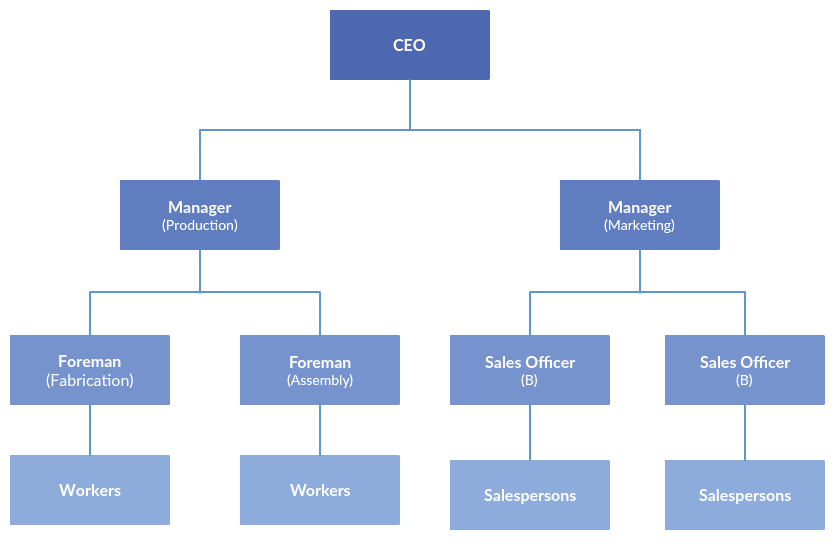
\includegraphics[scale=0.45]{gambar/struktur-organisasi.png}
	\caption{Struktur Organisasi PT. NASA}
	\label{fig:struktur_organisasi}
\end{figure}

Seperti yang bisa dilihat pada \ref{fig:struktur_organisasi}, \lipsum[1]
\vspace{0.5ex}
